\documentclass[1p]{elsarticle_modified}
%\bibliographystyle{elsarticle-num}

%\usepackage[colorlinks]{hyperref}
%\usepackage{abbrmath_seonhwa} %\Abb, \Ascr, \Acal ,\Abf, \Afrak
\usepackage{amsfonts}
\usepackage{amssymb}
\usepackage{amsmath}
\usepackage{amsthm}
\usepackage{scalefnt}
\usepackage{amsbsy}
\usepackage{kotex}
\usepackage{caption}
\usepackage{subfig}
\usepackage{color}
\usepackage{graphicx}
\usepackage{xcolor} %% white, black, red, green, blue, cyan, magenta, yellow
\usepackage{float}
\usepackage{setspace}
\usepackage{hyperref}

\usepackage{tikz}
\usetikzlibrary{arrows}

\usepackage{multirow}
\usepackage{array} % fixed length table
\usepackage{hhline}

%%%%%%%%%%%%%%%%%%%%%
\makeatletter
\renewcommand*\env@matrix[1][\arraystretch]{%
	\edef\arraystretch{#1}%
	\hskip -\arraycolsep
	\let\@ifnextchar\new@ifnextchar
	\array{*\c@MaxMatrixCols c}}
\makeatother %https://tex.stackexchange.com/questions/14071/how-can-i-increase-the-line-spacing-in-a-matrix
%%%%%%%%%%%%%%%

\usepackage[normalem]{ulem}

\newcommand{\msout}[1]{\ifmmode\text{\sout{\ensuremath{#1}}}\else\sout{#1}\fi}
%SOURCE: \msout is \stkout macro in https://tex.stackexchange.com/questions/20609/strikeout-in-math-mode

\newcommand{\cancel}[1]{
	\ifmmode
	{\color{red}\msout{#1}}
	\else
	{\color{red}\sout{#1}}
	\fi
}

\newcommand{\add}[1]{
	{\color{blue}\uwave{#1}}
}

\newcommand{\replace}[2]{
	\ifmmode
	{\color{red}\msout{#1}}{\color{blue}\uwave{#2}}
	\else
	{\color{red}\sout{#1}}{\color{blue}\uwave{#2}}
	\fi
}

\newcommand{\Sol}{\mathcal{S}} %segment
\newcommand{\D}{D} %diagram
\newcommand{\A}{\mathcal{A}} %arc


%%%%%%%%%%%%%%%%%%%%%%%%%%%%%5 test

\def\sl{\operatorname{\textup{SL}}(2,\Cbb)}
\def\psl{\operatorname{\textup{PSL}}(2,\Cbb)}
\def\quan{\mkern 1mu \triangleright \mkern 1mu}

\theoremstyle{definition}
\newtheorem{thm}{Theorem}[section]
\newtheorem{prop}[thm]{Proposition}
\newtheorem{lem}[thm]{Lemma}
\newtheorem{ques}[thm]{Question}
\newtheorem{cor}[thm]{Corollary}
\newtheorem{defn}[thm]{Definition}
\newtheorem{exam}[thm]{Example}
\newtheorem{rmk}[thm]{Remark}
\newtheorem{alg}[thm]{Algorithm}

\newcommand{\I}{\sqrt{-1}}
\begin{document}

%\begin{frontmatter}
%
%\title{Boundary parabolic representations of knots up to 8 crossings}
%
%%% Group authors per affiliation:
%\author{Yunhi Cho} 
%\address{Department of Mathematics, University of Seoul, Seoul, Korea}
%\ead{yhcho@uos.ac.kr}
%
%
%\author{Seonhwa Kim} %\fnref{s_kim}}
%\address{Center for Geometry and Physics, Institute for Basic Science, Pohang, 37673, Korea}
%\ead{ryeona17@ibs.re.kr}
%
%\author{Hyuk Kim}
%\address{Department of Mathematical Sciences, Seoul National University, Seoul 08826, Korea}
%\ead{hyukkim@snu.ac.kr}
%
%\author{Seokbeom Yoon}
%\address{Department of Mathematical Sciences, Seoul National University, Seoul, 08826,  Korea}
%\ead{sbyoon15@snu.ac.kr}
%
%\begin{abstract}
%We find all boundary parabolic representation of knots up to 8 crossings.
%
%\end{abstract}
%\begin{keyword}
%    \MSC[2010] 57M25 
%\end{keyword}
%
%\end{frontmatter}

%\linenumbers
%\tableofcontents
%
\newcommand\colored[1]{\textcolor{white}{\rule[-0.35ex]{0.8em}{1.4ex}}\kern-0.8em\color{red} #1}%
%\newcommand\colored[1]{\textcolor{white}{ #1}\kern-2.17ex	\textcolor{white}{ #1}\kern-1.81ex	\textcolor{white}{ #1}\kern-2.15ex\color{red}#1	}

{\Large $\underline{12n_{0700}~(K12n_{0700})}$}

\setlength{\tabcolsep}{10pt}
\renewcommand{\arraystretch}{1.6}
\vspace{1cm}\begin{tabular}{m{100pt}>{\centering\arraybackslash}m{274pt}}
\multirow{5}{120pt}{
	\centering
	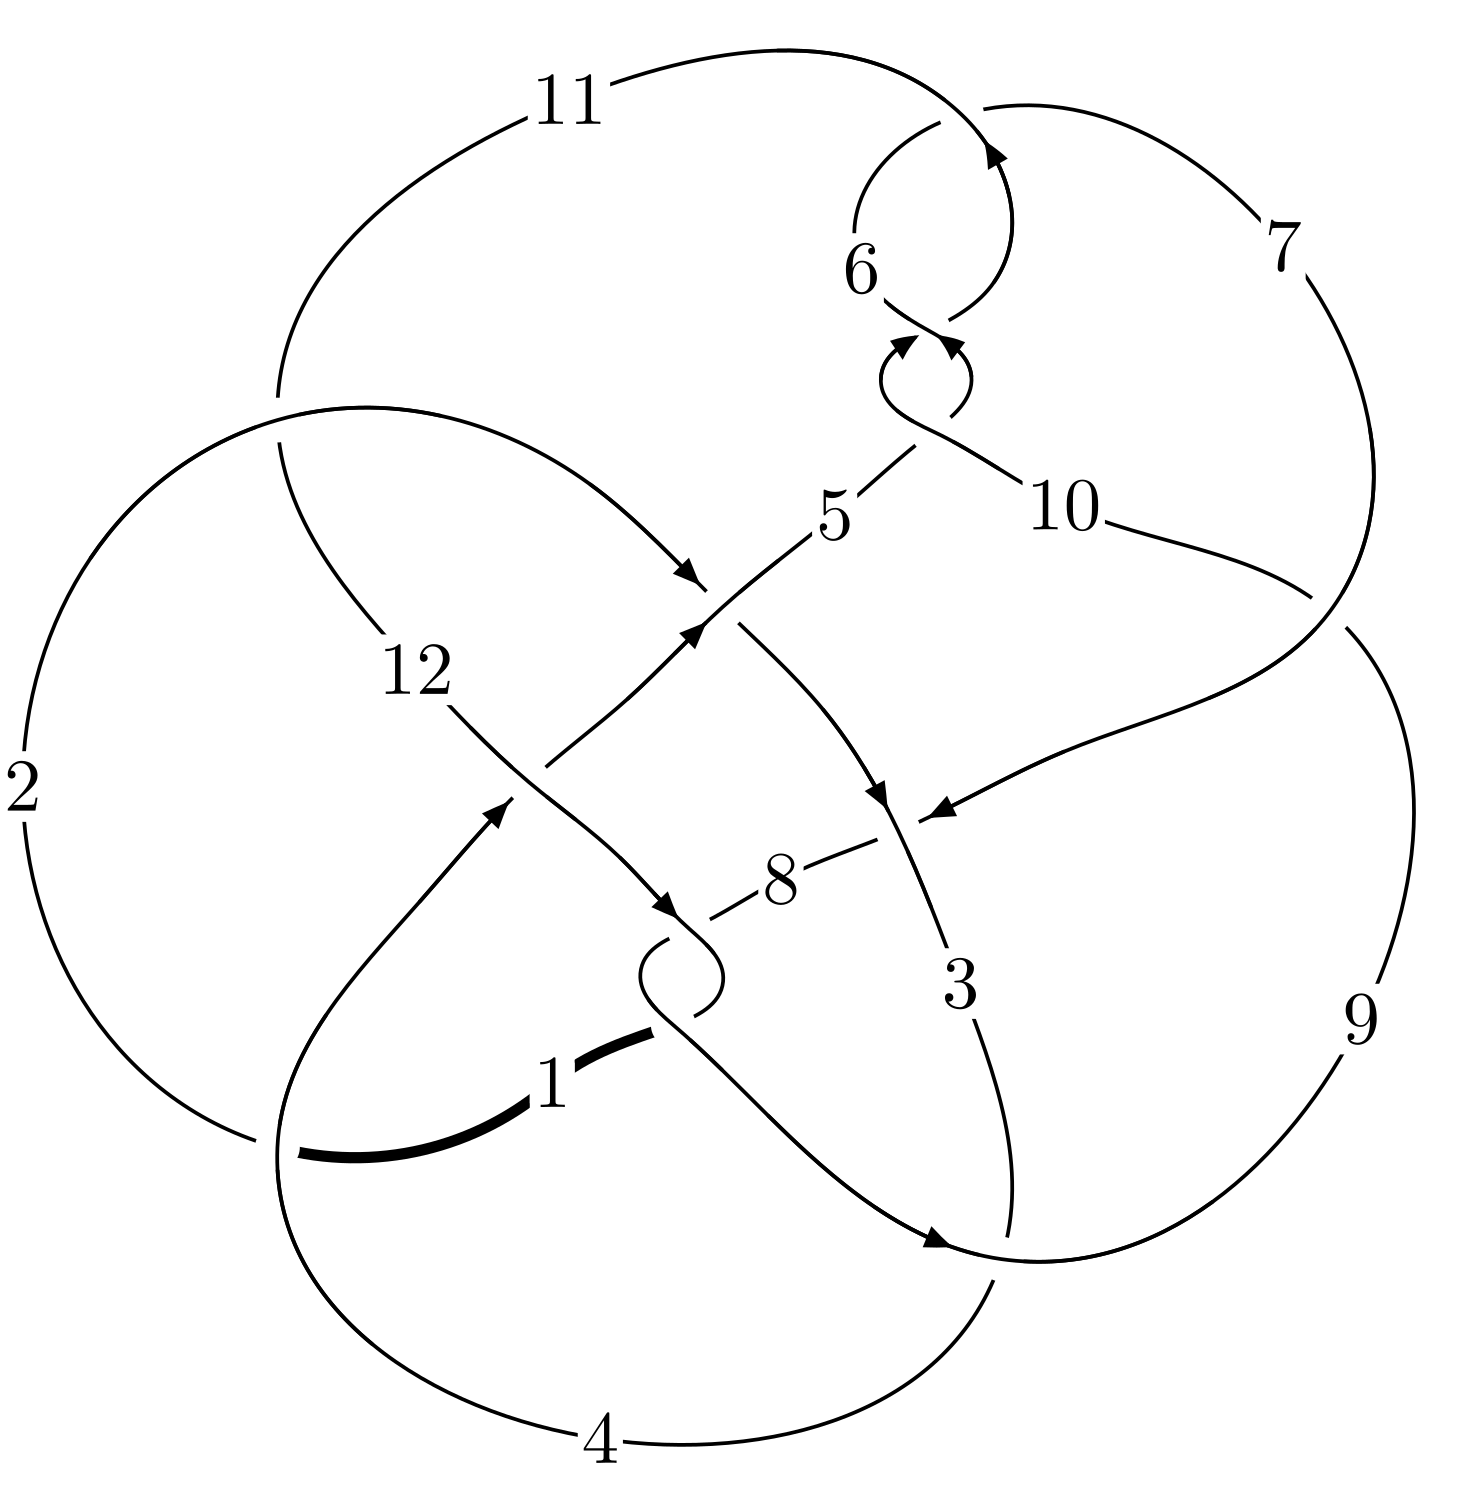
\includegraphics[width=112pt]{../../../GIT/diagram.site/Diagrams/png/2789_12n_0700.png}\\
\ \ \ A knot diagram\footnotemark}&
\allowdisplaybreaks
\textbf{Linearized knot diagam} \\
\cline{2-2}
 &
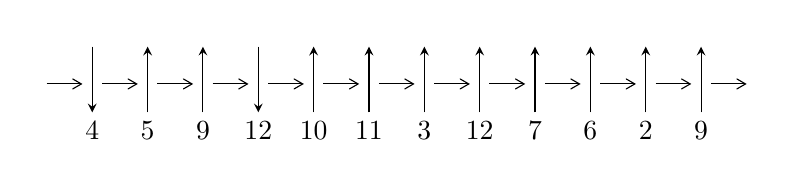
\begin{tikzpicture}[x=20pt, y=17pt]
	% nodes
	\node (C0) at (0, 0) {};
	\node (C1) at (1, 0) {};
	\node (C1U) at (1, +1) {};
	\node (C1D) at (1, -1) {4};

	\node (C2) at (2, 0) {};
	\node (C2U) at (2, +1) {};
	\node (C2D) at (2, -1) {5};

	\node (C3) at (3, 0) {};
	\node (C3U) at (3, +1) {};
	\node (C3D) at (3, -1) {9};

	\node (C4) at (4, 0) {};
	\node (C4U) at (4, +1) {};
	\node (C4D) at (4, -1) {12};

	\node (C5) at (5, 0) {};
	\node (C5U) at (5, +1) {};
	\node (C5D) at (5, -1) {10};

	\node (C6) at (6, 0) {};
	\node (C6U) at (6, +1) {};
	\node (C6D) at (6, -1) {11};

	\node (C7) at (7, 0) {};
	\node (C7U) at (7, +1) {};
	\node (C7D) at (7, -1) {3};

	\node (C8) at (8, 0) {};
	\node (C8U) at (8, +1) {};
	\node (C8D) at (8, -1) {12};

	\node (C9) at (9, 0) {};
	\node (C9U) at (9, +1) {};
	\node (C9D) at (9, -1) {7};

	\node (C10) at (10, 0) {};
	\node (C10U) at (10, +1) {};
	\node (C10D) at (10, -1) {6};

	\node (C11) at (11, 0) {};
	\node (C11U) at (11, +1) {};
	\node (C11D) at (11, -1) {2};

	\node (C12) at (12, 0) {};
	\node (C12U) at (12, +1) {};
	\node (C12D) at (12, -1) {9};
	\node (C13) at (13, 0) {};

	% arrows
	\draw[->,>={angle 60}]
	(C0) edge (C1) (C1) edge (C2) (C2) edge (C3) (C3) edge (C4) (C4) edge (C5) (C5) edge (C6) (C6) edge (C7) (C7) edge (C8) (C8) edge (C9) (C9) edge (C10) (C10) edge (C11) (C11) edge (C12) (C12) edge (C13) ;	\draw[->,>=stealth]
	(C1U) edge (C1D) (C2D) edge (C2U) (C3D) edge (C3U) (C4U) edge (C4D) (C5D) edge (C5U) (C6D) edge (C6U) (C7D) edge (C7U) (C8D) edge (C8U) (C9D) edge (C9U) (C10D) edge (C10U) (C11D) edge (C11U) (C12D) edge (C12U) ;
	\end{tikzpicture} \\
\hhline{~~} \\& 
\textbf{Solving Sequence} \\ \cline{2-2} 
 &
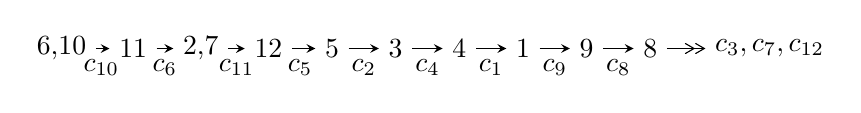
\begin{tikzpicture}[x=23pt, y=7pt]
	% node
	\node (A0) at (-1/8, 0) {6,10};
	\node (A1) at (1, 0) {11};
	\node (A2) at (33/16, 0) {2,7};
	\node (A3) at (25/8, 0) {12};
	\node (A4) at (33/8, 0) {5};
	\node (A5) at (41/8, 0) {3};
	\node (A6) at (49/8, 0) {4};
	\node (A7) at (57/8, 0) {1};
	\node (A8) at (65/8, 0) {9};
	\node (A9) at (73/8, 0) {8};
	\node (C1) at (1/2, -1) {$c_{10}$};
	\node (C2) at (3/2, -1) {$c_{6}$};
	\node (C3) at (21/8, -1) {$c_{11}$};
	\node (C4) at (29/8, -1) {$c_{5}$};
	\node (C5) at (37/8, -1) {$c_{2}$};
	\node (C6) at (45/8, -1) {$c_{4}$};
	\node (C7) at (53/8, -1) {$c_{1}$};
	\node (C8) at (61/8, -1) {$c_{9}$};
	\node (C9) at (69/8, -1) {$c_{8}$};
	\node (A10) at (11, 0) {$c_{3},c_{7},c_{12}$};

	% edge
	\draw[->,>=stealth]	
	(A0) edge (A1) (A1) edge (A2) (A2) edge (A3) (A3) edge (A4) (A4) edge (A5) (A5) edge (A6) (A6) edge (A7) (A7) edge (A8) (A8) edge (A9) ;
	\draw[->>,>={angle 60}]	
	(A9) edge (A10);
\end{tikzpicture} \\ 

\end{tabular} \\

\footnotetext{
The image of knot diagram is generated by the software ``\textbf{Draw programme}" developed by Andrew Bartholomew(\url{http://www.layer8.co.uk/maths/draw/index.htm\#Running-draw}), where we modified some parts for our purpose(\url{https://github.com/CATsTAILs/LinksPainter}).
}\phantom \\ \newline 
\centering \textbf{Ideals for irreducible components\footnotemark of $X_{\text{par}}$} 
 
\begin{align*}
I^u_{1}&=\langle 
12 u^{31}-42 u^{30}+\cdots+b+13,\;-13 u^{31}+41 u^{30}+\cdots+2 a-20,\;u^{32}-5 u^{31}+\cdots-8 u-2\rangle \\
I^u_{2}&=\langle 
-3 u^{15}-2 u^{14}+\cdots+b-3,\;3 u^{15}-22 u^{13}+\cdots+2 a+5,\;u^{16}+2 u^{15}+\cdots-3 u+2\rangle \\
I^u_{3}&=\langle 
- u^{14}- u^{13}+5 u^{12}+4 u^{11}-10 u^{10}-5 u^9+9 u^8-2 u^6+4 u^5-2 u^4-2 u^3- a u+b- u+1,\\
\phantom{I^u_{3}}&\phantom{= \langle  }- u^{14} a-5 u^{14}+\cdots+3 a+12,\\
\phantom{I^u_{3}}&\phantom{= \langle  }u^{15}+u^{14}-6 u^{13}-5 u^{12}+14 u^{11}+8 u^{10}-14 u^9- u^8+2 u^7-8 u^6+6 u^5+4 u^4-2 u^3+2 u^2-2 u-1\rangle \\
\\
\end{align*}
\raggedright * 3 irreducible components of $\dim_{\mathbb{C}}=0$, with total 78 representations.\\
\footnotetext{All coefficients of polynomials are rational numbers. But the coefficients are sometimes approximated in decimal forms when there is not enough margin.}
\newpage
\renewcommand{\arraystretch}{1}
\centering \section*{I. $I^u_{1}= \langle 12 u^{31}-42 u^{30}+\cdots+b+13,\;-13 u^{31}+41 u^{30}+\cdots+2 a-20,\;u^{32}-5 u^{31}+\cdots-8 u-2 \rangle$}
\flushleft \textbf{(i) Arc colorings}\\
\begin{tabular}{m{7pt} m{180pt} m{7pt} m{180pt} }
\flushright $a_{6}=$&$\begin{pmatrix}0\\u\end{pmatrix}$ \\
\flushright $a_{10}=$&$\begin{pmatrix}1\\0\end{pmatrix}$ \\
\flushright $a_{11}=$&$\begin{pmatrix}1\\- u^2\end{pmatrix}$ \\
\flushright $a_{2}=$&$\begin{pmatrix}\frac{13}{2} u^{31}-\frac{41}{2} u^{30}+\cdots+\frac{69}{2} u+10\\-12 u^{31}+42 u^{30}+\cdots-62 u-13\end{pmatrix}$ \\
\flushright $a_{7}=$&$\begin{pmatrix}u\\- u^3+u\end{pmatrix}$ \\
\flushright $a_{12}=$&$\begin{pmatrix}\frac{17}{2} u^{31}-\frac{61}{2} u^{30}+\cdots+\frac{103}{2} u+12\\-12 u^{31}+42 u^{30}+\cdots-79 u-17\end{pmatrix}$ \\
\flushright $a_{5}=$&$\begin{pmatrix}- u\\u\end{pmatrix}$ \\
\flushright $a_{3}=$&$\begin{pmatrix}-\frac{1}{2} u^{31}+\frac{15}{2} u^{30}+\cdots-\frac{49}{2} u-2\\-5 u^{31}+14 u^{30}+\cdots-3 u-1\end{pmatrix}$ \\
\flushright $a_{4}=$&$\begin{pmatrix}\frac{7}{2} u^{31}-\frac{15}{2} u^{30}+\cdots+\frac{15}{2} u+5\\-5 u^{31}+14 u^{30}+\cdots-3 u-1\end{pmatrix}$ \\
\flushright $a_{1}=$&$\begin{pmatrix}-\frac{9}{2} u^{31}+\frac{31}{2} u^{30}+\cdots-\frac{39}{2} u-5\\12 u^{31}-42 u^{30}+\cdots+79 u+17\end{pmatrix}$ \\
\flushright $a_{9}=$&$\begin{pmatrix}- u^4+u^2+1\\u^6-2 u^4+u^2\end{pmatrix}$ \\
\flushright $a_{8}=$&$\begin{pmatrix}-\frac{27}{2} u^{31}+\frac{99}{2} u^{30}+\cdots-\frac{199}{2} u-21\\19 u^{31}-71 u^{30}+\cdots+139 u+29\end{pmatrix}$\\&\end{tabular}
\flushleft \textbf{(ii) Obstruction class $= -1$}\\~\\
\flushleft \textbf{(iii) Cusp Shapes $= 19 u^{31}-65 u^{30}-138 u^{29}+623 u^{28}+427 u^{27}-2612 u^{26}-1023 u^{25}+6228 u^{24}+3091 u^{23}-8672 u^{22}-8566 u^{21}+4803 u^{20}+15237 u^{19}+6582 u^{18}-14312 u^{17}-16767 u^{16}+1566 u^{15}+14326 u^{14}+11332 u^{13}-1711 u^{12}-10557 u^{11}-6164 u^{10}+1148 u^9+3788 u^8+3056 u^7+240 u^6-1226 u^5-540 u^4-312 u^3+110 u^2+80 u+16$}\\~\\
\newpage\renewcommand{\arraystretch}{1}
\flushleft \textbf{(iv) u-Polynomials at the component}\newline \\
\begin{tabular}{m{50pt}|m{274pt}}
Crossings & \hspace{64pt}u-Polynomials at each crossing \\
\hline $$\begin{aligned}c_{1}\end{aligned}$$&$\begin{aligned}
&u^{32}-17 u^{31}+\cdots-308 u+178
\end{aligned}$\\
\hline $$\begin{aligned}c_{2},c_{11}\end{aligned}$$&$\begin{aligned}
&u^{32}+2 u^{31}+\cdots-11 u+1
\end{aligned}$\\
\hline $$\begin{aligned}c_{3},c_{8},c_{12}\end{aligned}$$&$\begin{aligned}
&u^{32}+23 u^{30}+\cdots+u-1
\end{aligned}$\\
\hline $$\begin{aligned}c_{4}\end{aligned}$$&$\begin{aligned}
&u^{32}+29 u^{31}+\cdots+393216 u+32768
\end{aligned}$\\
\hline $$\begin{aligned}c_{5},c_{6},c_{10}\end{aligned}$$&$\begin{aligned}
&u^{32}-5 u^{31}+\cdots-8 u-2
\end{aligned}$\\
\hline $$\begin{aligned}c_{7}\end{aligned}$$&$\begin{aligned}
&u^{32}+u^{31}+\cdots+221 u-97
\end{aligned}$\\
\hline $$\begin{aligned}c_{9}\end{aligned}$$&$\begin{aligned}
&u^{32}+15 u^{31}+\cdots+964 u+86
\end{aligned}$\\
\hline
\end{tabular}\\~\\
\newpage\renewcommand{\arraystretch}{1}
\flushleft \textbf{(v) Riley Polynomials at the component}\newline \\
\begin{tabular}{m{50pt}|m{274pt}}
Crossings & \hspace{64pt}Riley Polynomials at each crossing \\
\hline $$\begin{aligned}c_{1}\end{aligned}$$&$\begin{aligned}
&y^{32}-33 y^{31}+\cdots-1623172 y+31684
\end{aligned}$\\
\hline $$\begin{aligned}c_{2},c_{11}\end{aligned}$$&$\begin{aligned}
&y^{32}+14 y^{31}+\cdots-73 y+1
\end{aligned}$\\
\hline $$\begin{aligned}c_{3},c_{8},c_{12}\end{aligned}$$&$\begin{aligned}
&y^{32}+46 y^{31}+\cdots+13 y+1
\end{aligned}$\\
\hline $$\begin{aligned}c_{4}\end{aligned}$$&$\begin{aligned}
&y^{32}-9 y^{31}+\cdots-5368709120 y+1073741824
\end{aligned}$\\
\hline $$\begin{aligned}c_{5},c_{6},c_{10}\end{aligned}$$&$\begin{aligned}
&y^{32}-29 y^{31}+\cdots-60 y+4
\end{aligned}$\\
\hline $$\begin{aligned}c_{7}\end{aligned}$$&$\begin{aligned}
&y^{32}+25 y^{31}+\cdots-27307 y+9409
\end{aligned}$\\
\hline $$\begin{aligned}c_{9}\end{aligned}$$&$\begin{aligned}
&y^{32}+7 y^{31}+\cdots-138956 y+7396
\end{aligned}$\\
\hline
\end{tabular}\\~\\
\newpage\flushleft \textbf{(vi) Complex Volumes and Cusp Shapes}
$$\begin{array}{c|c|c}  
\text{Solutions to }I^u_{1}& \I (\text{vol} + \sqrt{-1}CS) & \text{Cusp shape}\\
 \hline 
\begin{aligned}
u &= -0.856862 + 0.544335 I \\
a &= -0.529669 + 0.145017 I \\
b &= -0.374915 + 0.412577 I\end{aligned}
 & -7.76454 - 4.88822 I & \phantom{-}4.38586 + 5.79440 I \\ \hline\begin{aligned}
u &= -0.856862 - 0.544335 I \\
a &= -0.529669 - 0.145017 I \\
b &= -0.374915 - 0.412577 I\end{aligned}
 & -7.76454 + 4.88822 I & \phantom{-}4.38586 - 5.79440 I \\ \hline\begin{aligned}
u &= -0.300083 + 0.868605 I \\
a &= \phantom{-}0.628210 + 0.007038 I \\
b &= \phantom{-}0.194628 - 0.543554 I\end{aligned}
 & -9.54364 - 0.04641 I & \phantom{-}0.192477 - 0.463915 I \\ \hline\begin{aligned}
u &= -0.300083 - 0.868605 I \\
a &= \phantom{-}0.628210 - 0.007038 I \\
b &= \phantom{-}0.194628 + 0.543554 I\end{aligned}
 & -9.54364 + 0.04641 I & \phantom{-}0.192477 + 0.463915 I \\ \hline\begin{aligned}
u &= -0.982425 + 0.459735 I \\
a &= \phantom{-}0.063117 - 0.663220 I \\
b &= -0.242898 - 0.680581 I\end{aligned}
 & -8.42524 + 6.40056 I & \phantom{-}6.06353 - 2.39705 I \\ \hline\begin{aligned}
u &= -0.982425 - 0.459735 I \\
a &= \phantom{-}0.063117 + 0.663220 I \\
b &= -0.242898 + 0.680581 I\end{aligned}
 & -8.42524 - 6.40056 I & \phantom{-}6.06353 + 2.39705 I \\ \hline\begin{aligned}
u &= -0.211672 + 0.838103 I \\
a &= -0.712628 - 1.047410 I \\
b &= -1.028680 + 0.375549 I\end{aligned}
 & -10.8094 - 11.0307 I & \phantom{-}3.82556 + 6.27574 I \\ \hline\begin{aligned}
u &= -0.211672 - 0.838103 I \\
a &= -0.712628 + 1.047410 I \\
b &= -1.028680 - 0.375549 I\end{aligned}
 & -10.8094 + 11.0307 I & \phantom{-}3.82556 - 6.27574 I \\ \hline\begin{aligned}
u &= -1.229180 + 0.220961 I \\
a &= \phantom{-}0.111894 + 0.489674 I \\
b &= \phantom{-}0.245737 + 0.577172 I\end{aligned}
 & \phantom{-}1.77560 + 0.48261 I & \phantom{-}9.87124 + 2.81544 I \\ \hline\begin{aligned}
u &= -1.229180 - 0.220961 I \\
a &= \phantom{-}0.111894 - 0.489674 I \\
b &= \phantom{-}0.245737 - 0.577172 I\end{aligned}
 & \phantom{-}1.77560 - 0.48261 I & \phantom{-}9.87124 - 2.81544 I\\
 \hline 
 \end{array}$$\newpage$$\begin{array}{c|c|c}  
\text{Solutions to }I^u_{1}& \I (\text{vol} + \sqrt{-1}CS) & \text{Cusp shape}\\
 \hline 
\begin{aligned}
u &= -1.262910 + 0.254948 I \\
a &= \phantom{-}0.070086 - 0.361128 I \\
b &= -0.003556 - 0.473942 I\end{aligned}
 & \phantom{-}1.17420 - 4.36507 I & \phantom{-}10.02842 + 6.42012 I \\ \hline\begin{aligned}
u &= -1.262910 - 0.254948 I \\
a &= \phantom{-}0.070086 + 0.361128 I \\
b &= -0.003556 + 0.473942 I\end{aligned}
 & \phantom{-}1.17420 + 4.36507 I & \phantom{-}10.02842 - 6.42012 I \\ \hline\begin{aligned}
u &= \phantom{-}1.287670 + 0.253472 I \\
a &= -1.52393 + 0.12920 I \\
b &= \phantom{-}1.99507 + 0.21991 I\end{aligned}
 & \phantom{-}1.37746 + 2.34487 I & \phantom{-}8.41481 - 0.55216 I \\ \hline\begin{aligned}
u &= \phantom{-}1.287670 - 0.253472 I \\
a &= -1.52393 - 0.12920 I \\
b &= \phantom{-}1.99507 - 0.21991 I\end{aligned}
 & \phantom{-}1.37746 - 2.34487 I & \phantom{-}8.41481 + 0.55216 I \\ \hline\begin{aligned}
u &= -0.098169 + 0.677929 I \\
a &= \phantom{-}0.71726 + 1.41090 I \\
b &= \phantom{-}1.026900 - 0.347744 I\end{aligned}
 & -1.60725 - 3.69611 I & \phantom{-}3.29803 + 2.27748 I \\ \hline\begin{aligned}
u &= -0.098169 - 0.677929 I \\
a &= \phantom{-}0.71726 - 1.41090 I \\
b &= \phantom{-}1.026900 + 0.347744 I\end{aligned}
 & -1.60725 + 3.69611 I & \phantom{-}3.29803 - 2.27748 I \\ \hline\begin{aligned}
u &= -0.015798 + 0.674807 I \\
a &= -0.638339 - 0.789035 I \\
b &= -0.542531 + 0.418291 I\end{aligned}
 & -2.66882 + 1.00290 I & \phantom{-}3.62847 - 3.27774 I \\ \hline\begin{aligned}
u &= -0.015798 - 0.674807 I \\
a &= -0.638339 + 0.789035 I \\
b &= -0.542531 - 0.418291 I\end{aligned}
 & -2.66882 - 1.00290 I & \phantom{-}3.62847 + 3.27774 I \\ \hline\begin{aligned}
u &= \phantom{-}1.342160 + 0.077096 I \\
a &= \phantom{-}1.55439 - 1.39862 I \\
b &= -2.19406 + 1.75733 I\end{aligned}
 & \phantom{-}5.49774 - 0.90354 I & \phantom{-}12.53276 + 1.80769 I \\ \hline\begin{aligned}
u &= \phantom{-}1.342160 - 0.077096 I \\
a &= \phantom{-}1.55439 + 1.39862 I \\
b &= -2.19406 - 1.75733 I\end{aligned}
 & \phantom{-}5.49774 + 0.90354 I & \phantom{-}12.53276 - 1.80769 I\\
 \hline 
 \end{array}$$\newpage$$\begin{array}{c|c|c}  
\text{Solutions to }I^u_{1}& \I (\text{vol} + \sqrt{-1}CS) & \text{Cusp shape}\\
 \hline 
\begin{aligned}
u &= \phantom{-}1.330040 + 0.281861 I \\
a &= \phantom{-}2.47693 - 0.37891 I \\
b &= -3.40120 - 0.19418 I\end{aligned}
 & \phantom{-}2.89499 + 7.19326 I & \phantom{-}8.98916 - 5.05295 I \\ \hline\begin{aligned}
u &= \phantom{-}1.330040 - 0.281861 I \\
a &= \phantom{-}2.47693 + 0.37891 I \\
b &= -3.40120 + 0.19418 I\end{aligned}
 & \phantom{-}2.89499 - 7.19326 I & \phantom{-}8.98916 + 5.05295 I \\ \hline\begin{aligned}
u &= \phantom{-}1.39497 + 0.35222 I \\
a &= -2.21296 + 0.14720 I \\
b &= \phantom{-}3.13885 + 0.57412 I\end{aligned}
 & -5.7214 + 15.3218 I & \phantom{-}8.04302 - 7.62554 I \\ \hline\begin{aligned}
u &= \phantom{-}1.39497 - 0.35222 I \\
a &= -2.21296 - 0.14720 I \\
b &= \phantom{-}3.13885 - 0.57412 I\end{aligned}
 & -5.7214 - 15.3218 I & \phantom{-}8.04302 + 7.62554 I \\ \hline\begin{aligned}
u &= \phantom{-}1.45144 + 0.37096 I \\
a &= \phantom{-}0.664841 + 0.529951 I \\
b &= -0.768383 - 1.015820 I\end{aligned}
 & -3.96493 + 4.54692 I & \phantom{-0.000000 } 0 \\ \hline\begin{aligned}
u &= \phantom{-}1.45144 - 0.37096 I \\
a &= \phantom{-}0.664841 - 0.529951 I \\
b &= -0.768383 + 1.015820 I\end{aligned}
 & -3.96493 - 4.54692 I & \phantom{-0.000000 } 0 \\ \hline\begin{aligned}
u &= \phantom{-}1.49869 + 0.06046 I \\
a &= -1.30572 - 0.89485 I \\
b &= \phantom{-}1.90276 + 1.42005 I\end{aligned}
 & \phantom{-}0.09897 + 6.38740 I & \phantom{-}10.66369 - 5.63916 I \\ \hline\begin{aligned}
u &= \phantom{-}1.49869 - 0.06046 I \\
a &= -1.30572 + 0.89485 I \\
b &= \phantom{-}1.90276 - 1.42005 I\end{aligned}
 & \phantom{-}0.09897 - 6.38740 I & \phantom{-}10.66369 + 5.63916 I \\ \hline\begin{aligned}
u &= \phantom{-}0.475802\phantom{ +0.000000I} \\
a &= -0.529412\phantom{ +0.000000I} \\
b &= \phantom{-}0.251895\phantom{ +0.000000I}\end{aligned}
 & \phantom{-}0.724697\phantom{ +0.000000I} & \phantom{-}12.9880\phantom{ +0.000000I} \\ \hline\begin{aligned}
u &= -1.57937\phantom{ +0.000000I} \\
a &= \phantom{-}0.0469240\phantom{ +0.000000I} \\
b &= \phantom{-}0.0741106\phantom{ +0.000000I}\end{aligned}
 & \phantom{-}7.86571\phantom{ +0.000000I} & -16.8850\phantom{ +0.000000I}\\
 \hline 
 \end{array}$$\newpage$$\begin{array}{c|c|c}  
\text{Solutions to }I^u_{1}& \I (\text{vol} + \sqrt{-1}CS) & \text{Cusp shape}\\
 \hline 
\begin{aligned}
u &= -0.296068 + 0.129818 I \\
a &= \phantom{-}0.37776 + 2.13705 I \\
b &= \phantom{-}0.389271 + 0.583672 I\end{aligned}
 & \phantom{-}0.49245 + 1.79175 I & \phantom{-}2.45715 - 5.83736 I \\ \hline\begin{aligned}
u &= -0.296068 - 0.129818 I \\
a &= \phantom{-}0.37776 - 2.13705 I \\
b &= \phantom{-}0.389271 - 0.583672 I\end{aligned}
 & \phantom{-}0.49245 - 1.79175 I & \phantom{-}2.45715 + 5.83736 I\\
 \hline 
 \end{array}$$\newpage\newpage\renewcommand{\arraystretch}{1}
\centering \section*{II. $I^u_{2}= \langle -3 u^{15}-2 u^{14}+\cdots+b-3,\;3 u^{15}-22 u^{13}+\cdots+2 a+5,\;u^{16}+2 u^{15}+\cdots-3 u+2 \rangle$}
\flushleft \textbf{(i) Arc colorings}\\
\begin{tabular}{m{7pt} m{180pt} m{7pt} m{180pt} }
\flushright $a_{6}=$&$\begin{pmatrix}0\\u\end{pmatrix}$ \\
\flushright $a_{10}=$&$\begin{pmatrix}1\\0\end{pmatrix}$ \\
\flushright $a_{11}=$&$\begin{pmatrix}1\\- u^2\end{pmatrix}$ \\
\flushright $a_{2}=$&$\begin{pmatrix}-\frac{3}{2} u^{15}+11 u^{13}+\cdots+4 u-\frac{5}{2}\\3 u^{15}+2 u^{14}+\cdots-7 u+3\end{pmatrix}$ \\
\flushright $a_{7}=$&$\begin{pmatrix}u\\- u^3+u\end{pmatrix}$ \\
\flushright $a_{12}=$&$\begin{pmatrix}\frac{1}{2} u^{15}-3 u^{13}+\cdots+2 u+\frac{1}{2}\\- u^{15}+7 u^{13}+\cdots+u-1\end{pmatrix}$ \\
\flushright $a_{5}=$&$\begin{pmatrix}- u\\u\end{pmatrix}$ \\
\flushright $a_{3}=$&$\begin{pmatrix}\frac{1}{2} u^{15}+2 u^{14}+\cdots-2 u-\frac{1}{2}\\u^{15}-7 u^{13}+\cdots- u+1\end{pmatrix}$ \\
\flushright $a_{4}=$&$\begin{pmatrix}-\frac{1}{2} u^{15}+u^{14}+\cdots+u-\frac{3}{2}\\u^{15}-7 u^{13}+\cdots- u+1\end{pmatrix}$ \\
\flushright $a_{1}=$&$\begin{pmatrix}\frac{3}{2} u^{15}+u^{14}+\cdots- u+\frac{3}{2}\\- u^{15}+7 u^{13}+\cdots+u-1\end{pmatrix}$ \\
\flushright $a_{9}=$&$\begin{pmatrix}- u^4+u^2+1\\u^6-2 u^4+u^2\end{pmatrix}$ \\
\flushright $a_{8}=$&$\begin{pmatrix}-\frac{7}{2} u^{15}-3 u^{14}+\cdots+13 u-\frac{11}{2}\\4 u^{15}+3 u^{14}+\cdots-16 u+7\end{pmatrix}$\\&\end{tabular}
\flushleft \textbf{(ii) Obstruction class $= 1$}\\~\\
\flushleft \textbf{(iii) Cusp Shapes $= 4 u^{15}+4 u^{14}-25 u^{13}-14 u^{12}+63 u^{11}-69 u^9+59 u^8+8 u^7-72 u^6+47 u^5-18 u^3+25 u^2-16 u+16$}\\~\\
\newpage\renewcommand{\arraystretch}{1}
\flushleft \textbf{(iv) u-Polynomials at the component}\newline \\
\begin{tabular}{m{50pt}|m{274pt}}
Crossings & \hspace{64pt}u-Polynomials at each crossing \\
\hline $$\begin{aligned}c_{1}\end{aligned}$$&$\begin{aligned}
&u^{16}-14 u^{15}+\cdots-41 u+4
\end{aligned}$\\
\hline $$\begin{aligned}c_{2},c_{11}\end{aligned}$$&$\begin{aligned}
&u^{16}+2 u^{15}+\cdots+2 u+1
\end{aligned}$\\
\hline $$\begin{aligned}c_{3},c_{8}\end{aligned}$$&$\begin{aligned}
&u^{16}+6 u^{14}+\cdots+4 u+1
\end{aligned}$\\
\hline $$\begin{aligned}c_{4}\end{aligned}$$&$\begin{aligned}
&u^{16}+2 u^{15}+\cdots+2 u+1
\end{aligned}$\\
\hline $$\begin{aligned}c_{5},c_{6}\end{aligned}$$&$\begin{aligned}
&u^{16}-2 u^{15}+\cdots+3 u+2
\end{aligned}$\\
\hline $$\begin{aligned}c_{7}\end{aligned}$$&$\begin{aligned}
&u^{16}- u^{15}+\cdots+u^2+1
\end{aligned}$\\
\hline $$\begin{aligned}c_{9}\end{aligned}$$&$\begin{aligned}
&u^{16}-6 u^{15}+\cdots-7 u+2
\end{aligned}$\\
\hline $$\begin{aligned}c_{10}\end{aligned}$$&$\begin{aligned}
&u^{16}+2 u^{15}+\cdots-3 u+2
\end{aligned}$\\
\hline $$\begin{aligned}c_{12}\end{aligned}$$&$\begin{aligned}
&u^{16}+6 u^{14}+\cdots-4 u+1
\end{aligned}$\\
\hline
\end{tabular}\\~\\
\newpage\renewcommand{\arraystretch}{1}
\flushleft \textbf{(v) Riley Polynomials at the component}\newline \\
\begin{tabular}{m{50pt}|m{274pt}}
Crossings & \hspace{64pt}Riley Polynomials at each crossing \\
\hline $$\begin{aligned}c_{1}\end{aligned}$$&$\begin{aligned}
&y^{16}-16 y^{15}+\cdots-97 y+16
\end{aligned}$\\
\hline $$\begin{aligned}c_{2},c_{11}\end{aligned}$$&$\begin{aligned}
&y^{16}-4 y^{15}+\cdots-8 y+1
\end{aligned}$\\
\hline $$\begin{aligned}c_{3},c_{8},c_{12}\end{aligned}$$&$\begin{aligned}
&y^{16}+12 y^{15}+\cdots-10 y+1
\end{aligned}$\\
\hline $$\begin{aligned}c_{4}\end{aligned}$$&$\begin{aligned}
&y^{16}-8 y^{15}+\cdots-4 y+1
\end{aligned}$\\
\hline $$\begin{aligned}c_{5},c_{6},c_{10}\end{aligned}$$&$\begin{aligned}
&y^{16}-16 y^{15}+\cdots- y+4
\end{aligned}$\\
\hline $$\begin{aligned}c_{7}\end{aligned}$$&$\begin{aligned}
&y^{16}+15 y^{15}+\cdots+2 y+1
\end{aligned}$\\
\hline $$\begin{aligned}c_{9}\end{aligned}$$&$\begin{aligned}
&y^{16}-6 y^{14}+\cdots+7 y+4
\end{aligned}$\\
\hline
\end{tabular}\\~\\
\newpage\flushleft \textbf{(vi) Complex Volumes and Cusp Shapes}
$$\begin{array}{c|c|c}  
\text{Solutions to }I^u_{2}& \I (\text{vol} + \sqrt{-1}CS) & \text{Cusp shape}\\
 \hline 
\begin{aligned}
u &= \phantom{-}1.137400 + 0.146818 I \\
a &= -0.149955 + 0.449115 I \\
b &= -0.236497 + 0.488807 I\end{aligned}
 & \phantom{-}1.79945 - 1.49089 I & \phantom{-}10.63523 + 4.79741 I \\ \hline\begin{aligned}
u &= \phantom{-}1.137400 - 0.146818 I \\
a &= -0.149955 - 0.449115 I \\
b &= -0.236497 - 0.488807 I\end{aligned}
 & \phantom{-}1.79945 + 1.49089 I & \phantom{-}10.63523 - 4.79741 I \\ \hline\begin{aligned}
u &= \phantom{-}0.199163 + 0.721319 I \\
a &= -0.606622 + 1.036950 I \\
b &= -0.868785 - 0.231047 I\end{aligned}
 & -0.63802 + 4.76461 I & \phantom{-}9.16165 - 6.96874 I \\ \hline\begin{aligned}
u &= \phantom{-}0.199163 - 0.721319 I \\
a &= -0.606622 - 1.036950 I \\
b &= -0.868785 + 0.231047 I\end{aligned}
 & -0.63802 - 4.76461 I & \phantom{-}9.16165 + 6.96874 I \\ \hline\begin{aligned}
u &= -1.242630 + 0.215465 I \\
a &= \phantom{-}2.27494 + 1.85843 I \\
b &= -3.22733 - 1.81917 I\end{aligned}
 & -4.26568 - 2.08418 I & \phantom{-}10.49854 + 3.93307 I \\ \hline\begin{aligned}
u &= -1.242630 - 0.215465 I \\
a &= \phantom{-}2.27494 - 1.85843 I \\
b &= -3.22733 + 1.81917 I\end{aligned}
 & -4.26568 + 2.08418 I & \phantom{-}10.49854 - 3.93307 I \\ \hline\begin{aligned}
u &= \phantom{-}0.571020 + 0.339582 I \\
a &= \phantom{-}0.039795 + 0.842875 I \\
b &= -0.263501 + 0.494812 I\end{aligned}
 & \phantom{-}1.12725 - 1.33975 I & \phantom{-}12.02351 + 1.24817 I \\ \hline\begin{aligned}
u &= \phantom{-}0.571020 - 0.339582 I \\
a &= \phantom{-}0.039795 - 0.842875 I \\
b &= -0.263501 - 0.494812 I\end{aligned}
 & \phantom{-}1.12725 + 1.33975 I & \phantom{-}12.02351 - 1.24817 I \\ \hline\begin{aligned}
u &= -0.141358 + 0.640937 I \\
a &= -0.679498 - 1.144790 I \\
b &= \phantom{-}0.829793 - 0.273689 I\end{aligned}
 & -7.63694 - 0.91148 I & \phantom{-}3.93951 + 0.55564 I \\ \hline\begin{aligned}
u &= -0.141358 - 0.640937 I \\
a &= -0.679498 + 1.144790 I \\
b &= \phantom{-}0.829793 + 0.273689 I\end{aligned}
 & -7.63694 + 0.91148 I & \phantom{-}3.93951 - 0.55564 I\\
 \hline 
 \end{array}$$\newpage$$\begin{array}{c|c|c}  
\text{Solutions to }I^u_{2}& \I (\text{vol} + \sqrt{-1}CS) & \text{Cusp shape}\\
 \hline 
\begin{aligned}
u &= \phantom{-}1.369690 + 0.297062 I \\
a &= \phantom{-}0.132211 - 0.195026 I \\
b &= \phantom{-}0.239022 - 0.227851 I\end{aligned}
 & -2.78866 + 4.38420 I & \phantom{-}9.70308 - 2.57288 I \\ \hline\begin{aligned}
u &= \phantom{-}1.369690 - 0.297062 I \\
a &= \phantom{-}0.132211 + 0.195026 I \\
b &= \phantom{-}0.239022 + 0.227851 I\end{aligned}
 & -2.78866 - 4.38420 I & \phantom{-}9.70308 + 2.57288 I \\ \hline\begin{aligned}
u &= -1.376870 + 0.303108 I \\
a &= -1.97992 - 0.37746 I \\
b &= \phantom{-}2.84050 - 0.08041 I\end{aligned}
 & \phantom{-}4.35415 - 8.50155 I & \phantom{-}13.9603 + 7.3316 I \\ \hline\begin{aligned}
u &= -1.376870 - 0.303108 I \\
a &= -1.97992 + 0.37746 I \\
b &= \phantom{-}2.84050 + 0.08041 I\end{aligned}
 & \phantom{-}4.35415 + 8.50155 I & \phantom{-}13.9603 - 7.3316 I \\ \hline\begin{aligned}
u &= -1.51641 + 0.01833 I \\
a &= -0.780954 - 0.139106 I \\
b &= \phantom{-}1.186800 + 0.196628 I\end{aligned}
 & \phantom{-}8.04846 + 0.00268 I & \phantom{-}26.0782 - 3.0287 I \\ \hline\begin{aligned}
u &= -1.51641 - 0.01833 I \\
a &= -0.780954 + 0.139106 I \\
b &= \phantom{-}1.186800 - 0.196628 I\end{aligned}
 & \phantom{-}8.04846 - 0.00268 I & \phantom{-}26.0782 + 3.0287 I\\
 \hline 
 \end{array}$$\newpage\newpage\renewcommand{\arraystretch}{1}
\centering \section*{III. $I^u_{3}= \langle - u^{14}- u^{13}+\cdots+b+1,\;- u^{14} a-5 u^{14}+\cdots+3 a+12,\;u^{15}+u^{14}+\cdots-2 u-1 \rangle$}
\flushleft \textbf{(i) Arc colorings}\\
\begin{tabular}{m{7pt} m{180pt} m{7pt} m{180pt} }
\flushright $a_{6}=$&$\begin{pmatrix}0\\u\end{pmatrix}$ \\
\flushright $a_{10}=$&$\begin{pmatrix}1\\0\end{pmatrix}$ \\
\flushright $a_{11}=$&$\begin{pmatrix}1\\- u^2\end{pmatrix}$ \\
\flushright $a_{2}=$&$\begin{pmatrix}a\\u^{14}+u^{13}+\cdots+u-1\end{pmatrix}$ \\
\flushright $a_{7}=$&$\begin{pmatrix}u\\- u^3+u\end{pmatrix}$ \\
\flushright $a_{12}=$&$\begin{pmatrix}u^{13} a+u^{14}+\cdots+a-1\\- u^{13} a- u^{12} a+\cdots- a-1\end{pmatrix}$ \\
\flushright $a_{5}=$&$\begin{pmatrix}- u\\u\end{pmatrix}$ \\
\flushright $a_{3}=$&$\begin{pmatrix}u^{14}+u^{13}+\cdots+a+u\\- u^{12}- u^{11}+\cdots+a u-1\end{pmatrix}$ \\
\flushright $a_{4}=$&$\begin{pmatrix}u^{13} a+u^{14}+\cdots+a-1\\- u^{13} a- u^{12} a+\cdots- a-1\end{pmatrix}$ \\
\flushright $a_{1}=$&$\begin{pmatrix}-2 u^{13} a- u^{14}+\cdots- a+2\\2 u^{13} a+u^{13}+\cdots+2 a+1\end{pmatrix}$ \\
\flushright $a_{9}=$&$\begin{pmatrix}- u^4+u^2+1\\u^6-2 u^4+u^2\end{pmatrix}$ \\
\flushright $a_{8}=$&$\begin{pmatrix}-3 u^{14}+u^{13}+\cdots+a+6\\2 u^{14}-2 u^{13}+\cdots- a u-3\end{pmatrix}$\\&\end{tabular}
\flushleft \textbf{(ii) Obstruction class $= -1$}\\~\\
\flushleft \textbf{(iii) Cusp Shapes $= 4 u^{12}-20 u^{10}+4 u^9+36 u^8-16 u^7-20 u^6+20 u^5-12 u^4-4 u^3+12 u^2-4 u+6$}\\~\\
\newpage\renewcommand{\arraystretch}{1}
\flushleft \textbf{(iv) u-Polynomials at the component}\newline \\
\begin{tabular}{m{50pt}|m{274pt}}
Crossings & \hspace{64pt}u-Polynomials at each crossing \\
\hline $$\begin{aligned}c_{1}\end{aligned}$$&$\begin{aligned}
&(u^{15}+13 u^{14}+\cdots+8 u-1)^{2}
\end{aligned}$\\
\hline $$\begin{aligned}c_{2},c_{11}\end{aligned}$$&$\begin{aligned}
&u^{30}+13 u^{29}+\cdots-198 u-23
\end{aligned}$\\
\hline $$\begin{aligned}c_{3},c_{8},c_{12}\end{aligned}$$&$\begin{aligned}
&u^{30}- u^{29}+\cdots+356 u+599
\end{aligned}$\\
\hline $$\begin{aligned}c_{4}\end{aligned}$$&$\begin{aligned}
&(u-1)^{30}
\end{aligned}$\\
\hline $$\begin{aligned}c_{5},c_{6},c_{10}\end{aligned}$$&$\begin{aligned}
&(u^{15}+u^{14}+\cdots-2 u-1)^{2}
\end{aligned}$\\
\hline $$\begin{aligned}c_{7}\end{aligned}$$&$\begin{aligned}
&u^{30}+u^{29}+\cdots+48394 u-9199
\end{aligned}$\\
\hline $$\begin{aligned}c_{9}\end{aligned}$$&$\begin{aligned}
&(u^{15}-3 u^{14}+\cdots+4 u^2-1)^{2}
\end{aligned}$\\
\hline
\end{tabular}\\~\\
\newpage\renewcommand{\arraystretch}{1}
\flushleft \textbf{(v) Riley Polynomials at the component}\newline \\
\begin{tabular}{m{50pt}|m{274pt}}
Crossings & \hspace{64pt}Riley Polynomials at each crossing \\
\hline $$\begin{aligned}c_{1}\end{aligned}$$&$\begin{aligned}
&(y^{15}-29 y^{14}+\cdots+8 y-1)^{2}
\end{aligned}$\\
\hline $$\begin{aligned}c_{2},c_{11}\end{aligned}$$&$\begin{aligned}
&y^{30}-5 y^{29}+\cdots+7808 y+529
\end{aligned}$\\
\hline $$\begin{aligned}c_{3},c_{8},c_{12}\end{aligned}$$&$\begin{aligned}
&y^{30}+39 y^{29}+\cdots+402780 y+358801
\end{aligned}$\\
\hline $$\begin{aligned}c_{4}\end{aligned}$$&$\begin{aligned}
&(y-1)^{30}
\end{aligned}$\\
\hline $$\begin{aligned}c_{5},c_{6},c_{10}\end{aligned}$$&$\begin{aligned}
&(y^{15}-13 y^{14}+\cdots+8 y-1)^{2}
\end{aligned}$\\
\hline $$\begin{aligned}c_{7}\end{aligned}$$&$\begin{aligned}
&y^{30}+27 y^{29}+\cdots-796940 y+84621601
\end{aligned}$\\
\hline $$\begin{aligned}c_{9}\end{aligned}$$&$\begin{aligned}
&(y^{15}+7 y^{14}+\cdots+8 y-1)^{2}
\end{aligned}$\\
\hline
\end{tabular}\\~\\
\newpage\flushleft \textbf{(vi) Complex Volumes and Cusp Shapes}
$$\begin{array}{c|c|c}  
\text{Solutions to }I^u_{3}& \I (\text{vol} + \sqrt{-1}CS) & \text{Cusp shape}\\
 \hline 
\begin{aligned}
u &= \phantom{-}0.897290 + 0.288232 I \\
a &= -0.503485 - 0.559425 I \\
b &= \phantom{-}0.416988 - 0.227974 I\end{aligned}
 & \phantom{-}0.184105 - 0.159076 I & \phantom{-}5.79403 - 0.85194 I \\ \hline\begin{aligned}
u &= \phantom{-}0.897290 + 0.288232 I \\
a &= -0.347272 + 0.365622 I \\
b &= \phantom{-}0.290527 + 0.647087 I\end{aligned}
 & \phantom{-}0.184105 - 0.159076 I & \phantom{-}5.79403 - 0.85194 I \\ \hline\begin{aligned}
u &= \phantom{-}0.897290 - 0.288232 I \\
a &= -0.503485 + 0.559425 I \\
b &= \phantom{-}0.416988 + 0.227974 I\end{aligned}
 & \phantom{-}0.184105 + 0.159076 I & \phantom{-}5.79403 + 0.85194 I \\ \hline\begin{aligned}
u &= \phantom{-}0.897290 - 0.288232 I \\
a &= -0.347272 - 0.365622 I \\
b &= \phantom{-}0.290527 - 0.647087 I\end{aligned}
 & \phantom{-}0.184105 + 0.159076 I & \phantom{-}5.79403 + 0.85194 I \\ \hline\begin{aligned}
u &= \phantom{-}0.200931 + 0.760138 I \\
a &= \phantom{-}0.347773 - 0.900603 I \\
b &= \phantom{-}0.695074 + 0.555297 I\end{aligned}
 & -2.05700 + 4.11725 I & \phantom{-}2.59688 - 3.71929 I \\ \hline\begin{aligned}
u &= \phantom{-}0.200931 + 0.760138 I \\
a &= -0.908735 + 0.674195 I \\
b &= -0.754461 - 0.083397 I\end{aligned}
 & -2.05700 + 4.11725 I & \phantom{-}2.59688 - 3.71929 I \\ \hline\begin{aligned}
u &= \phantom{-}0.200931 - 0.760138 I \\
a &= \phantom{-}0.347773 + 0.900603 I \\
b &= \phantom{-}0.695074 - 0.555297 I\end{aligned}
 & -2.05700 - 4.11725 I & \phantom{-}2.59688 + 3.71929 I \\ \hline\begin{aligned}
u &= \phantom{-}0.200931 - 0.760138 I \\
a &= -0.908735 - 0.674195 I \\
b &= -0.754461 + 0.083397 I\end{aligned}
 & -2.05700 - 4.11725 I & \phantom{-}2.59688 + 3.71929 I \\ \hline\begin{aligned}
u &= -1.224710 + 0.250895 I \\
a &= \phantom{-}2.08574 + 1.21971 I \\
b &= -3.86630 - 0.92593 I\end{aligned}
 & -5.28079 - 1.64925 I & \phantom{-}1.60633 + 0.16522 I \\ \hline\begin{aligned}
u &= -1.224710 + 0.250895 I \\
a &= -2.88112 - 1.34627 I \\
b &= \phantom{-}2.86043 + 0.97048 I\end{aligned}
 & -5.28079 - 1.64925 I & \phantom{-}1.60633 + 0.16522 I\\
 \hline 
 \end{array}$$\newpage$$\begin{array}{c|c|c}  
\text{Solutions to }I^u_{3}& \I (\text{vol} + \sqrt{-1}CS) & \text{Cusp shape}\\
 \hline 
\begin{aligned}
u &= -1.224710 - 0.250895 I \\
a &= \phantom{-}2.08574 - 1.21971 I \\
b &= -3.86630 + 0.92593 I\end{aligned}
 & -5.28079 + 1.64925 I & \phantom{-}1.60633 - 0.16522 I \\ \hline\begin{aligned}
u &= -1.224710 - 0.250895 I \\
a &= -2.88112 + 1.34627 I \\
b &= \phantom{-}2.86043 - 0.97048 I\end{aligned}
 & -5.28079 + 1.64925 I & \phantom{-}1.60633 - 0.16522 I \\ \hline\begin{aligned}
u &= -0.074720 + 0.708028 I \\
a &= \phantom{-}0.611710 + 0.650680 I \\
b &= -1.60975 - 0.81488 I\end{aligned}
 & -8.75399 - 1.81248 I & -1.85619 + 4.33913 I \\ \hline\begin{aligned}
u &= -0.074720 + 0.708028 I \\
a &= \phantom{-}0.90095 - 2.36865 I \\
b &= \phantom{-}0.506407 - 0.384488 I\end{aligned}
 & -8.75399 - 1.81248 I & -1.85619 + 4.33913 I \\ \hline\begin{aligned}
u &= -0.074720 - 0.708028 I \\
a &= \phantom{-}0.611710 - 0.650680 I \\
b &= -1.60975 + 0.81488 I\end{aligned}
 & -8.75399 + 1.81248 I & -1.85619 - 4.33913 I \\ \hline\begin{aligned}
u &= -0.074720 - 0.708028 I \\
a &= \phantom{-}0.90095 + 2.36865 I \\
b &= \phantom{-}0.506407 + 0.384488 I\end{aligned}
 & -8.75399 + 1.81248 I & -1.85619 - 4.33913 I \\ \hline\begin{aligned}
u &= \phantom{-}1.30332\phantom{ +0.000000I} \\
a &= -1.64310 + 0.40643 I \\
b &= \phantom{-}2.14148 + 0.52971 I\end{aligned}
 & -1.05425\phantom{ +0.000000I} & \phantom{-}9.03940\phantom{ +0.000000I} \\ \hline\begin{aligned}
u &= \phantom{-}1.30332\phantom{ +0.000000I} \\
a &= -1.64310 - 0.40643 I \\
b &= \phantom{-}2.14148 - 0.52971 I\end{aligned}
 & -1.05425\phantom{ +0.000000I} & \phantom{-}9.03940\phantom{ +0.000000I} \\ \hline\begin{aligned}
u &= \phantom{-}1.314200 + 0.295245 I \\
a &= -0.346248 + 1.242720 I \\
b &= \phantom{-}1.35266 - 2.62536 I\end{aligned}
 & -4.39644 + 5.45324 I & \phantom{-}3.99532 - 6.35130 I \\ \hline\begin{aligned}
u &= \phantom{-}1.314200 + 0.295245 I \\
a &= -0.55258 + 2.12183 I \\
b &= \phantom{-}0.82195 - 1.53095 I\end{aligned}
 & -4.39644 + 5.45324 I & \phantom{-}3.99532 - 6.35130 I\\
 \hline 
 \end{array}$$\newpage$$\begin{array}{c|c|c}  
\text{Solutions to }I^u_{3}& \I (\text{vol} + \sqrt{-1}CS) & \text{Cusp shape}\\
 \hline 
\begin{aligned}
u &= \phantom{-}1.314200 - 0.295245 I \\
a &= -0.346248 - 1.242720 I \\
b &= \phantom{-}1.35266 + 2.62536 I\end{aligned}
 & -4.39644 - 5.45324 I & \phantom{-}3.99532 + 6.35130 I \\ \hline\begin{aligned}
u &= \phantom{-}1.314200 - 0.295245 I \\
a &= -0.55258 - 2.12183 I \\
b &= \phantom{-}0.82195 + 1.53095 I\end{aligned}
 & -4.39644 - 5.45324 I & \phantom{-}3.99532 + 6.35130 I \\ \hline\begin{aligned}
u &= -1.378140 + 0.316043 I \\
a &= -1.70922 - 0.18417 I \\
b &= \phantom{-}2.62416 - 0.47024 I\end{aligned}
 & \phantom{-}2.93922 - 8.01682 I & \phantom{-}7.04132 + 4.89679 I \\ \hline\begin{aligned}
u &= -1.378140 + 0.316043 I \\
a &= \phantom{-}1.88334 + 0.09068 I \\
b &= -2.41375 + 0.28637 I\end{aligned}
 & \phantom{-}2.93922 - 8.01682 I & \phantom{-}7.04132 + 4.89679 I \\ \hline\begin{aligned}
u &= -1.378140 - 0.316043 I \\
a &= -1.70922 + 0.18417 I \\
b &= \phantom{-}2.62416 + 0.47024 I\end{aligned}
 & \phantom{-}2.93922 + 8.01682 I & \phantom{-}7.04132 - 4.89679 I \\ \hline\begin{aligned}
u &= -1.378140 - 0.316043 I \\
a &= \phantom{-}1.88334 - 0.09068 I \\
b &= -2.41375 - 0.28637 I\end{aligned}
 & \phantom{-}2.93922 + 8.01682 I & \phantom{-}7.04132 - 4.89679 I \\ \hline\begin{aligned}
u &= -1.43385\phantom{ +0.000000I} \\
a &= -1.16104\phantom{ +0.000000I} \\
b &= \phantom{-}1.90536\phantom{ +0.000000I}\end{aligned}
 & \phantom{-}7.22226\phantom{ +0.000000I} & \phantom{-}9.97710\phantom{ +0.000000I} \\ \hline\begin{aligned}
u &= -1.43385\phantom{ +0.000000I} \\
a &= \phantom{-}1.32884\phantom{ +0.000000I} \\
b &= -1.66477\phantom{ +0.000000I}\end{aligned}
 & \phantom{-}7.22226\phantom{ +0.000000I} & \phantom{-}9.97710\phantom{ +0.000000I} \\ \hline\begin{aligned}
u &= -0.339181\phantom{ +0.000000I} \\
a &= -2.02164 + 3.01582 I \\
b &= -0.685704 - 1.022910 I\end{aligned}
 & -5.98181\phantom{ +0.000000I} & \phantom{-}8.62820\phantom{ +0.000000I} \\ \hline\begin{aligned}
u &= -0.339181\phantom{ +0.000000I} \\
a &= -2.02164 - 3.01582 I \\
b &= -0.685704 + 1.022910 I\end{aligned}
 & -5.98181\phantom{ +0.000000I} & \phantom{-}8.62820\phantom{ +0.000000I}\\
 \hline 
 \end{array}$$\newpage
\newpage\renewcommand{\arraystretch}{1}
\centering \section*{ IV. u-Polynomials}
\begin{tabular}{m{50pt}|m{274pt}}
Crossings & \hspace{64pt}u-Polynomials at each crossing \\
\hline $$\begin{aligned}c_{1}\end{aligned}$$&$\begin{aligned}
&((u^{15}+13 u^{14}+\cdots+8 u-1)^{2})(u^{16}-14 u^{15}+\cdots-41 u+4)\\
&\cdot(u^{32}-17 u^{31}+\cdots-308 u+178)
\end{aligned}$\\
\hline $$\begin{aligned}c_{2},c_{11}\end{aligned}$$&$\begin{aligned}
&(u^{16}+2 u^{15}+\cdots+2 u+1)(u^{30}+13 u^{29}+\cdots-198 u-23)\\
&\cdot(u^{32}+2 u^{31}+\cdots-11 u+1)
\end{aligned}$\\
\hline $$\begin{aligned}c_{3},c_{8}\end{aligned}$$&$\begin{aligned}
&(u^{16}+6 u^{14}+\cdots+4 u+1)(u^{30}- u^{29}+\cdots+356 u+599)\\
&\cdot(u^{32}+23 u^{30}+\cdots+u-1)
\end{aligned}$\\
\hline $$\begin{aligned}c_{4}\end{aligned}$$&$\begin{aligned}
&((u-1)^{30})(u^{16}+2 u^{15}+\cdots+2 u+1)\\
&\cdot(u^{32}+29 u^{31}+\cdots+393216 u+32768)
\end{aligned}$\\
\hline $$\begin{aligned}c_{5},c_{6}\end{aligned}$$&$\begin{aligned}
&((u^{15}+u^{14}+\cdots-2 u-1)^{2})(u^{16}-2 u^{15}+\cdots+3 u+2)\\
&\cdot(u^{32}-5 u^{31}+\cdots-8 u-2)
\end{aligned}$\\
\hline $$\begin{aligned}c_{7}\end{aligned}$$&$\begin{aligned}
&(u^{16}- u^{15}+\cdots+u^2+1)(u^{30}+u^{29}+\cdots+48394 u-9199)\\
&\cdot(u^{32}+u^{31}+\cdots+221 u-97)
\end{aligned}$\\
\hline $$\begin{aligned}c_{9}\end{aligned}$$&$\begin{aligned}
&((u^{15}-3 u^{14}+\cdots+4 u^2-1)^{2})(u^{16}-6 u^{15}+\cdots-7 u+2)\\
&\cdot(u^{32}+15 u^{31}+\cdots+964 u+86)
\end{aligned}$\\
\hline $$\begin{aligned}c_{10}\end{aligned}$$&$\begin{aligned}
&((u^{15}+u^{14}+\cdots-2 u-1)^{2})(u^{16}+2 u^{15}+\cdots-3 u+2)\\
&\cdot(u^{32}-5 u^{31}+\cdots-8 u-2)
\end{aligned}$\\
\hline $$\begin{aligned}c_{12}\end{aligned}$$&$\begin{aligned}
&(u^{16}+6 u^{14}+\cdots-4 u+1)(u^{30}- u^{29}+\cdots+356 u+599)\\
&\cdot(u^{32}+23 u^{30}+\cdots+u-1)
\end{aligned}$\\
\hline
\end{tabular}\newpage\renewcommand{\arraystretch}{1}
\centering \section*{ V. Riley Polynomials}
\begin{tabular}{m{50pt}|m{274pt}}
Crossings & \hspace{64pt}Riley Polynomials at each crossing \\
\hline $$\begin{aligned}c_{1}\end{aligned}$$&$\begin{aligned}
&((y^{15}-29 y^{14}+\cdots+8 y-1)^{2})(y^{16}-16 y^{15}+\cdots-97 y+16)\\
&\cdot(y^{32}-33 y^{31}+\cdots-1623172 y+31684)
\end{aligned}$\\
\hline $$\begin{aligned}c_{2},c_{11}\end{aligned}$$&$\begin{aligned}
&(y^{16}-4 y^{15}+\cdots-8 y+1)(y^{30}-5 y^{29}+\cdots+7808 y+529)\\
&\cdot(y^{32}+14 y^{31}+\cdots-73 y+1)
\end{aligned}$\\
\hline $$\begin{aligned}c_{3},c_{8},c_{12}\end{aligned}$$&$\begin{aligned}
&(y^{16}+12 y^{15}+\cdots-10 y+1)(y^{30}+39 y^{29}+\cdots+402780 y+358801)\\
&\cdot(y^{32}+46 y^{31}+\cdots+13 y+1)
\end{aligned}$\\
\hline $$\begin{aligned}c_{4}\end{aligned}$$&$\begin{aligned}
&((y-1)^{30})(y^{16}-8 y^{15}+\cdots-4 y+1)\\
&\cdot(y^{32}-9 y^{31}+\cdots-5368709120 y+1073741824)
\end{aligned}$\\
\hline $$\begin{aligned}c_{5},c_{6},c_{10}\end{aligned}$$&$\begin{aligned}
&((y^{15}-13 y^{14}+\cdots+8 y-1)^{2})(y^{16}-16 y^{15}+\cdots- y+4)\\
&\cdot(y^{32}-29 y^{31}+\cdots-60 y+4)
\end{aligned}$\\
\hline $$\begin{aligned}c_{7}\end{aligned}$$&$\begin{aligned}
&(y^{16}+15 y^{15}+\cdots+2 y+1)\\
&\cdot(y^{30}+27 y^{29}+\cdots-796940 y+84621601)\\
&\cdot(y^{32}+25 y^{31}+\cdots-27307 y+9409)
\end{aligned}$\\
\hline $$\begin{aligned}c_{9}\end{aligned}$$&$\begin{aligned}
&((y^{15}+7 y^{14}+\cdots+8 y-1)^{2})(y^{16}-6 y^{14}+\cdots+7 y+4)\\
&\cdot(y^{32}+7 y^{31}+\cdots-138956 y+7396)
\end{aligned}$\\
\hline
\end{tabular}
\vskip 2pc
\end{document}